\chapter{Style Analyser}
\label{cap:analyser}

In order to generate messages with the user's writing style, it is necessary to define parameters which will determine and describe it. For this purpose, we have developed a style analyser that extracts the messages written by the user and obtains the value of various metrics from them. Then it will be useful for analysing different user's emails and drawing conclusions about what parameters describe the writing style of each person more accurately.

In this section we are going to explain the architecture of this analyser (see Section \ref{ssection:stylearch}) and each of the modules that compose it (they are explained in Sections \ref{ssection:extmod}, \ref{ssection:prepmod}, \ref{ssection:typomod} and \ref{ssection:measmod}). Finally, we are going to discuss the obtained results and analyse them for drawing a conclusion (this discussion can be looked up in \ref{ssection:resconc}).

\section{Architecture} \label{ssection:stylearch}
The first step when we are designing a system's architecture is to know its input and output. In this case, we want to implement a natural language processing system that analyses the writing style of emails. As we have previously mentioned, the writing style analysis will be represented through chosen metrics. Therefore, our system's output is going to be that chosen metrics (they are explained in section \ref{ssection:measmod}).

In respect of the system's input, because of the nature of the problem we face, it is reasonable to think that it must be a single email. However, we do not have the corpus of emails to analyse. For this reason, our first step will be to extract the emails that will be analysed. Hence, our system's input is going to be the Gmail user for accessing to the information that we are interested in. Therefore, we are going to develop a system which receives a Gmail user as input and obtains different metrics of each message sent by the given user as output.

Once we clearly know the input and output of our system, we need to define the different steps that a message have to take for being analysed. In this way, we are going to design a pipeline architecture with four different phases (extraction, preprocess, typographic correction and measuring) as Figure \ref{fig:arch} shows. Thus, we divide the original job in 4 different and more simple tasks with distinct inputs and outputs required.

\begin{figure}[h]
	\centering%
	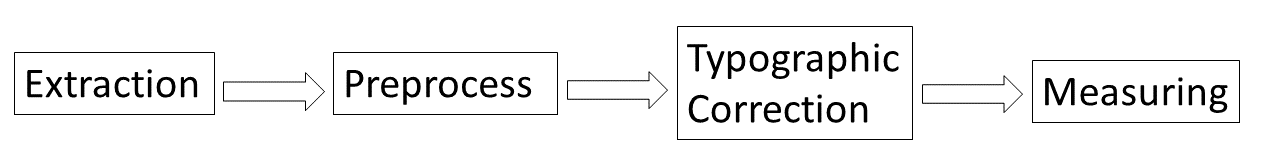
\includegraphics[width = 1\textwidth]{Imagenes/Bitmap/architecture.png}%
	\caption{Pipeline architecture of the style analyser}%
	\label{fig:arch}
\end{figure}

As it is easy to deduce, each of these phases is going to be developed as a different module. This implementation will have the advantage that each module is going to be able to work independently from the other modules, which will allow them to work in parallel. That is to say, while a message is being extracted, other e-mails could be being preprocessed, corrected or measured if they have gone through the previous phases.Let us now briefly explain what each of the defined phases consists of.

The first step, extraction phase, as the reader can imagine, consists of the extraction of each one of the sent messages of the given user. In this task, we are going to take advantage of all the studied concepts about the Gmail API (see Section \ref{ssect:gmailapi}) and make use of every resource it provides us. Besides, we will try to minimize the consumed quota units in each extraction, which means we will only make the requests to the Google Servers that are strictly necessary. This first step is not just the task of extracting the resource that represents each sent message from the user's account, but also the job of transforming it to the format that the preprocessing module needs. Hence, the input of this module will be the same input as that of the complete system (a Gmail user) and its output will be an extracted message ready for being preprocessed.

As for the second step, the preprocessing phase, consists of the modifying the extracted message so that it can be interpreted by the spaCy's natural language processing model to be used. Some of the changes that a message could suffer in this phase are: the removal of the signature, the disposal of the replied messages which appears under the text, the elimination of soft break lines that quoted-printable codification (see Section \ref{sssect:quot-p}) introduce in some messages, etc.

\section{Extracting Module} \label{ssection:extmod}

\section{Preprocessing Module} \label{ssection:prepmod}

\section{Typographic Correction Module} \label{ssection:typomod}

\section{Measuring module} \label{ssection:measmod}

As in our case we have used 31 lexical-syntactic features (due to previous studies, such as \cite{homem2011authorship}, yield encouraging results with lexical-syntactic features), following the classification of \cite{abbasi2008writeprints} (which categorised stylistic features as lexical, syntactic, structural, content-specific and idiosyncratic style markers), we will now divide them into 4 categories in which we have grouped them according to their usefulness in terms of what type of conclusions we can infer from each of them. These categories are: part of speech features (see Section \ref{sssect:posf}), punctuation features (see Section \ref{sssect:punctf}), vocabulary features (see Section \ref{sssect:vocabf}) and structural features (see Section \ref{sssect:strucf}). We must not confuse this latter category (which it belongs to the lexical features of the classification given in \cite{abbasi2008writeprints}) with the structural metrics explained in \cite{abbasi2008writeprints}.

Some of the popular metrics which are not used in this work, belong to the structural, content-specific and idiosyncratic style markers of \cite{abbasi2008writeprints}, but there are others which belong to the same categories as the explained metrics (lexical and syntactic).

\subsection{Part of Speech features}\label{sssect:posf}

We will call our part of speech metrics as the syntactic features which have to do with the part of speech of each word of the e-mails. Following the suggestion of \cite{holmes1985analysis}, we count the number of nouns, verbs, adjectives, adverbs, pronouns, determinants, conjunctions and prepositions of each text. By calculating this, significant stylistic traits may be found, because as \cite{somers1966statistical} claims: ``A more cultivated intellectual habit of thinking can increase the number of substantives used, while a more dynamic empathy and attitude can be habitually expressed by means of an increased number of verbs. It is also possible to detect a number of idiosyncrasies in the use of prepositions, subordinations, conjunctions and articles''.

In adding to this metrics, we calculate the verb-adjective ratio and the determinant-pronouns ratio, extracted from \cite{antosch1969diagnosis} and \cite{brainerd1974weighting}, respectively.

\subsection{Punctuation features}\label{sssect:punctf}

In order to extract conclusions from this syntactic features, and following the example of \cite{calix2008stylometry}, we calculate the amount of commas, periods, semi-colons, ellipsis and pair of brackets. With these metrics we can reach conclusions such as the structural complexity of a message (since, for example, juxtaposition structures appear in the presence of some of these scores), the division into sentences of the message or the need for clarification of the text transmitted (for example, by analysing the amount of brackets).

\subsection{Vocabulary features}\label{sssect:vocabf}

In terms of the vocabulary used, we work with the ``bag of words'' metrics, in other words, we note how many times each different word is used in a message. Of course this is not the only metric that we can categorise as a vocabulary feature and from which we can extract conclusions about the vocabulary used. There are many other which tries to set the parameters of, for instance, the difficult of the vocabulary or its richness. Besides, from the computing of the bag of words, we are able to easily obtain other style marker chosen which also belongs to this category of vocabulary features: the amount of different words in each text.

As for the difficulty level, it determines the level of education that someone needs to have if they are to understand the text. There are several indices available to calculate this level, such as the proposed in \cite{dale1948formula}, the Gunning Fog Index \citep{wiki:gunning} or the Flesch-Kincaid index \citep{dubay2004principles}, although the latter is the most commonly documented and cited. The expression which determines the Flesch-Kincaid index is the following:

$$
I_{FK} = 1.599\lambda-1.015\beta-31.517
$$

Where $\lambda$ is the mean of one-syllable words per 100 words, and $\beta$ is the mean sentence length measured by the number of words. However, as our spaCy's pretrained Spanish model (see Section \ref{sect:spacy}) is not able to divide words by syllables, we determine $\lambda$ as the mean of words with two or less characters per 100 words.

In respect of the richness of the vocabulary, we have chosen two different metrics. The first that we are going to explain is the one proposed by \cite{honore1979some}, which determines the richness of te vocabulary based on the total unrepeated words used in the text. The following formula defines it:

$$
R_H = \frac{100\log(M)}{M^2}
$$

Where $M$ is the number of different words in the text. However, as \cite{ril2014determination} claims, depending on the type of document being analysed, the calculation of $R_H$ has more or less validity (for instance, certain specialist articles, as their nature, requires constant repetition of words). As a consequence of this, another definition of richness of vocabulary is proposed by \cite{yule2014statistical}. This richness marker, that we are going to use as our second richness of vocabulary style marker, is called Yule's characteristic and defined with the following expression:

$$
K = \frac{10^4\left(\sum_{i = 1}^\infty i^2V_i-M\right)}{M^2}
$$

Where $M$ is the number of different words in the text and $V_i$ is the number of words that appear i times in the document.

From Yule's Characteristic we are able to calculate the Simpson's Index (denoted as $D$), defined in \cite{simpson1949measurement}. This famous metric is understood as the measurement of diversity based on the change that the two members of an arbitrary chosen pair of word tokens will belong to the same type. To calculate $D$ it is necessary to divide the total number of identical pairs in the sample by the number of all possible pairs, that is to say, what the following expression defines:

$$
D = \frac{\sum_{i = 1}^\infty i(i-1)V_i}{M(M-1)}
$$

Where we are maintaining the Yule's Characteristic notation. However, as we have transmitted in advance, it is possible to calculate the Simpson's Index if we know the value of Yule's Characteristic. This relationship is defined by the following expression (and we are going to use it in the implementation in order to speed the computing):

$$
10^{-4}K=D\left(1-\frac{1}{M}\right)
$$

Vocabulary distribution can also be measured by using a concept linguists have borrowed from thermodynamics and applied to communication theory: entropy (used in \cite{holmes1985analysis}). In literary text it is true that with an increase in internal structure, entropy decreases, and with an increase in disorder or randomness, the measure of entropy increases. The expression for the entropy of a system (vocabulary in this case) is:

$$
H = -\sum_{i=1}^{\infty} p_i\log(p_i)
$$

Where $p_i$ is the probability of appearance of the ith lemma (found by dividing the number of occurrences of that lemma by the total number of words in the text). Due to the value will change according to how much text is analysed, the formula may be refined in order that works of different length may be compared. In this way, as it is proposed in \cite{holmes1985analysis}, the following expression determines absolute diversity for any length text as 100, while absolute uniformity remains zero:

$$
H=-100\sum_{i = 1}^{\infty}p_i\frac{\log(p_i)}{\log(M)}
$$

In addition to the words distribution features (which are the bag of words and the amount of different words), the level of difficulty, the richness of vocabulary (which is measured by the formula proposed in \cite{honore1979some} and the Yule's Characteristic), the diversity (represented by the Simpson's Index) and the internal structure of the vocabulary (which is measured by the entropy), we have defined other three style markers which also allow us to extract conclusions about some feature of the vocabulary of the message. First of these is the most popular and old style marker: the mean word length. Researches as \cite{ril2014determination} claim that it is ``directly connected with the richness of the author's vocabulary and measures his or her ability to use complex words'', due to it is considered that complex words are formed by three or more syllables that do not represent proper nouns, prefixes, suffixes or compound words. Thus, \cite{ril2014determination} propose an expression similar to the following one in order to calculate it:

$$
L_W = \frac{\sum_{i=1}^{\infty}i*C_i}{N}\cdot 100
$$

Where $C_i$ is the number of words with $i$ characters and $N$ is the number of words used. This formula is analogous to the expression proposed by \cite{ril2014determination}, except that with the one that we have presented the punctuation marks are removed from the numerator.

\subsection{Structural features}\label{sssect:strucf}

\section{Results and conclusions} \label{ssection:resconc}
